\newpage
\subsection{Signalaufbereitung}
\label{subsec:pre_amplifier}
Aufgrund der Leitungsdämpfung muss die Amplitude des modulierten Signals vor der Filterung durch den Rekonstruktionsfilter verstärkt werden (siehe Kapitel \ref{subsec:receiver_schematic} - Abbildung \ref{fig:basic_schematic}: \textsc{Postamp}).Das Signal wird über einen nicht-invertierenden Verstärker aufbereitet:
\begin{figure}[H]
\centering
 
\includegraphics[scale=0.40]{gfx/preamp}
	\caption{Vorverstärker}
\end{figure}
Damit die Schaltung für verschiedene Leitungslängen skalierbar ist, wurde eine variable Verstärkung bis zu einem Faktor von $V_u = 500$ gewählt. 
\begin{figure}[H]
\begin{minipage}{0.45\textwidth} 
	\begin{align}
	V_U&=1+\frac{R_4}{R_5}\\
	\frac{R_4}{R_5} &>> 1\\
	V_U&\approx\frac{R_4}{R_5} \label{eq1}
	\end{align}
	\end{minipage}
	\hfill
\begin{minipage}{0.45\textwidth}
		% \textwidth bezieht sich nun auf die Minipage
Für große Verstärkungen errechnet(siehe Formel\ref{eq1}\footnotemark) ist die 1 beim Nicht-Invertierenden Verstärker zu vernachlässligen. Die Verstärkung berechnet sich lediglich aus den beiden Widerständen $R_{5}$ und $R_{4}$. 
\end{minipage}
\end{figure}
\noindent
Mit $0\Omega < R_4 < 500k\Omega$ und $R_5=1k\Omega$ ist die Verstärkung von 0 bis 500 einstellbar.
\\

\footnotetext{Quelle: Elektronik Vorlesungssunterlagen, Prof. Dr. Ralf Patz}
\begin{floatingfigure}[r]{7cm}
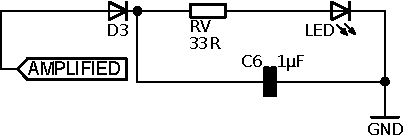
\includegraphics[width=6.5cm]{gfx/detect.pdf}
\caption{Signaldetektion}
\label{fig:detect}
\end{floatingfigure}
\noindent
Neben der Signalaufbereitung für die folgende Demodulation, wird das ver\-stär\-kte Signal auch für eine Signaldetektion aufbereitet. Zur Signalisierung wird eine Leuchtdiode an der Ge\-häu\-se\-front verwendet. Zur Glät\-tung der Spannung wird ein Kondensator parallel zu der Leuchtdiode mit Vorwiderstand geschaltet. Eine weitere Aufbereitung ist an dieser Stelle nicht notwendig, da das Trägersignal, als auch das Nachrichtensignal $\geq 50 Hz$  ist und somit für das menschliche Auge kein Flackern auftritt. 